%\documentclass{book}
\documentclass{report}

\pagenumbering{roman} 
\pagestyle{empty}

% Notas de aula
%
% Template criado em 24/9/2013
% Daniel Oliveira Dantas
%
% Ctrl+x 8 , c = ç

\usepackage[utf8]{inputenc}
\usepackage[english, brazil]{babel}

\usepackage{listings}
\lstset{
  language=C,                % choose the language of the code
  numbers=none,                   % where to put the line-numbers
  stepnumber=1,                   % the step between two line-numbers.        
  numbersep=10pt,                  % how far the line-numbers are from the code
  %backgroundcolor=\color{white},  % choose the background color. You must add \usepackage{color}
  showspaces=false,               % show spaces adding particular underscores
  showstringspaces=false,         % underline spaces within strings
  showtabs=false,                 % show tabs within strings adding particular underscores
  tabsize=2,                      % sets default tabsize to 2 spaces
  captionpos=b,                   % sets the caption-position to bottom
  breaklines=true,                % sets automatic line breaking
  breakatwhitespace=true,         % sets if automatic breaks should only happen at whitespace
  title=\lstname,                 % show the filename of files included with \lstinputlisting;
}

% Adicionado para permitir a criação de listas com vários graus de aninhamento
% ddantas, 24/03/2020
\usepackage{amssymb}
\usepackage{amsmath}
\usepackage[ampersand]{easylist}
\ListProperties(Hide=100, Hang=true, Progressive=3ex, Style*=--- ,
Style2*=$\bullet$ ,Style3*=$\circ$ ,Style4*=\tiny$\blacksquare$ )

% Adicionado para permitir a inserção de figuras
% ddantas, 24/03/2020
\usepackage{graphicx}


%formatacao

\newcommand{\TAB}{{\hspace*{1cm}}}
\newcommand{\NEWLINE}{~\\}
\newcommand{\BV}{\begin{verbatim}}
\newcommand{\EV}{\end{verbatim}}

%tipos de dados

\newcommand{\VOID}{{\tt void}}
\newcommand{\CHAR}{{\tt char}}
\newcommand{\INT}{{\tt int}}
\newcommand{\FLOAT}{{\tt float}}
\newcommand{\DOUBLE}{{\tt double}}

\newcommand{\LONGINT}{{\tt long int}}

%operadores

\newcommand{\AND}{{\tt \&\&}}
\newcommand{\OR}{{\tt ||}}

\newcommand{\LNOT}{{\tt \~{}}}
\newcommand{\LAND}{{\tt \&}}
\newcommand{\LOR}{{\tt |}}
\newcommand{\LXOR}{{\tt \^{}}}

%palavras reservadas

\newcommand{\IF}{{\tt if}}
\newcommand{\ELSE}{{\tt else}}

\newcommand{\SWITCH}{{\tt switch}}
\newcommand{\CASE}{{\tt case}}

\newcommand{\FOR}{{\tt for}}
\newcommand{\WHILE}{{\tt while}}

\newcommand{\BREAK}{{\tt break}}

\newcommand{\TRUE}{{\tt true}}
\newcommand{\FALSE}{{\tt false}}

\newcommand{\MAIN}{{\tt main}}

\newcommand{\SIZEOF}{{\tt sizeof}}

% funcoes

\newcommand{\SIN}{{\tt sin}}
\newcommand{\COS}{{\tt cos}}
\newcommand{\TAN}{{\tt tan}}
\newcommand{\LOG}{{\tt log}}

\newcommand{\PRINTF}{{\tt printf}}
\newcommand{\SCANF}{{\tt scanf}}

\newcommand{\SPRINTF}{{\tt sprintf}}
\newcommand{\SSCANF}{{\tt sscanf}}

\newcommand{\FPRINTF}{{\tt fprintf}}
\newcommand{\FSCANF}{{\tt fscanf}}

\newcommand{\GETS}{{\tt gets}}
\newcommand{\FGETS}{{\tt fgets}}

\newcommand{\FOPEN}{{\tt fopen}}
\newcommand{\FCLOSE}{{\tt fclose}}

\newcommand{\SYSTEM}{{\tt system}}

%renewcommand

\renewcommand\chaptername{Capítulo}
\renewcommand\lstlistingname{Listagem}



\title{Notas de aula de Processamento de imagens e Visão Computacional}
\author{Daniel Oliveira Dantas}
\date{24 de março de 2020}
\begin{document}

\maketitle

%%%%%%%%%%%%%%%%%%%%%%%%%%%%%%%%%%%%%%%%%%%%%%%%%%%%%%%%%%%%
%Índice
%%%%%%%%%%%%%%%%%%%%%%%%%%%%%%%%%%%%%%%%%%%%%%%%%%%%%%%%%%%%

\tableofcontents
\pagestyle{plain}


%%%%%%%%%%%%%%%%%%%%%%%%%%%%%%%%%%%%%%%%%%%%%%%%%%%%%%%%%%%%
%Capítulo: Introdução
%%%%%%%%%%%%%%%%%%%%%%%%%%%%%%%%%%%%%%%%%%%%%%%%%%%%%%%%%%%%

\chapter{Introdução}


\setcounter{page}{1}    % set page to 1 again to start arabic count
\pagenumbering{arabic}


Capítulo 1 de Gonzalez, \textit{Digital Image Processing}~\cite{gonzalez2006image}.

%%%%%%%%%%%%%%%%%%%%%%%%%%%%%%%%%%%%%%%%%%%%%%%%%%%%%%%%%%%%
\section{O que é processamento de imagens}

\begin{easylist}
  & O que é uma imagem?
  && Uma matriz
  && Uma função
  && Esses conceitos podem ser generalizados para mais dimensões
  & Uma definição de processamento de imagens: processo em que tanto a entrada quanto a saída são imagens.
  && Essa definição não engloba, porém, processos como valor médio da imagem, extração de pontos característicos, alguns tipos de reconstrução 3D, aplicações de segurança que detectam atividades suspeitas, reconhecimento de gestos, reconhecimento de caracteres (OCR) e outras aplicações consideradas do campo de visão computacional.
  & Uma definição mais abrangente: processos de baixo, médio e alto nível em que tanto a entrada quanto a saída são imagens.
  && Baixo nível: envolve operações primitivas, de redução de ruído, aumento de contraste, aumento de nitidez (\textit{sharpening}), \textit{thresholding} etc. Nos processos de baixo nível, tanto a entrada quanto a saída são imagens.
  && Médio nível: envolve tarefas como segmentação (particionamento), redução dos objetos a uma descrição ou formato apropriado para processamento, classificação (reconhecimento) de objetos. A entrada são imagens, e a saída são atributos extraídos dessas imagens, como bordas, contornos, características ou classe de objetos individuais.
  && Alto nível: envolve atividades cognitivas associadas com a visão. Cognição envolve atividades como memória, compreensão, aprendizado, raciocínio, atenção, resolução de problemas e tomada de decisão.
\end{easylist}

%%%%%%%%%%%%%%%%%%%%%%%%%%%%%%%%%%%%%%%%%%%%%%%%%%%%%%%%%%%%
\section{Origens do processamento digital de imagens}

\begin{easylist}
  & 1920: \textit{Bartlane cable picture transmission system}, 5 tons de cinza.
  & 1929: idem, 15 tons de cinza.
  & 1948: invenção do transistor.
  & 1950 a 1960: invenção das linguagens de programação de alto nível, COBOL e Fortran.
  & 1958: invenção do circuito integrado.
  & 1964: primeira foto da Lua tirada de uma sonda.
  & 1968 a 1971: invenção dos primeiros microprocessadores, CADC, TMS1000, 4004.
  & 1969: invenção do CCD.
  & 1971: primeira tomografia computadorizada
\end{easylist}

%%%%%%%%%%%%%%%%%%%%%%%%%%%%%%%%%%%%%%%%%%%%%%%%%%%%%%%%%%%%
\section{Áreas que usam processamento digital de imagens}

\begin{easylist}
  & Medicina, astronomia, meteorologia, indústria, fotografia, editoração, segurança etc.
  & Técnicas de obtenção de imagem:
  && Eletromagnética: luz, radiação UV, radiação IR, raios X, raios gama, microondas.
  && Eletrônica: microscopia eletrônica.
  && Mecânica: ondas acústicas, ultrassom.
  && Sintética: computação gráfica, fractais.
\end{easylist}

%%%%%%%%%%%%%%%%%%%%%%%%%%%%%%%%%%%%%%%%%%%%%%%%%%%%%%%%%%%%
\section{Passos fundamentais no processamento digital de imagens}

\begin{easylist}
& Aquisição
& Melhoramento (\textit{image enhancement)}
& Restauração
& Processamento de cores
& \textit{Wavelets} e processamento multirresolução
& Compressão
& Processamento morfológico
& Segmentação
& Representação e descrição
& Reconhecimento de objetos
\end{easylist}


%%%%%%%%%%%%%%%%%%%%%%%%%%%%%%%%%%%%%%%%%%%%%%%%%%%%%%%%%%%%
\section{Componentes de um sistema de processamento de imagens}

\begin{easylist}
& Sensores + \textit{hardware} especializado
& Computador + GPU
& Armazenamento em massa
& \textit{Software} de processamento de imagens
& Monitor de imagem
& Impressora
& Rede
\end{easylist}



%%%%%%%%%%%%%%%%%%%%%%%%%%%%%%%%%%%%%%%%%%%%%%%%%%%%%%%%%%%%
%Capítulo: Fundamentos de imagens digitais
%%%%%%%%%%%%%%%%%%%%%%%%%%%%%%%%%%%%%%%%%%%%%%%%%%%%%%%%%%%%

\chapter{Fundamentos de imagens digitais}

Capítulo 2 de Gonzalez, \textit{Digital Image Processing}~\cite{gonzalez2006image}.

%%%%%%%%%%%%%%%%%%%%%%%%%%%%%%%%%%%%%%%%%%%%%%%%%%%%%%%%%%%%
\section{Elementos de percepção visual}

%%%%%%%%%%%%%%%%%%%%%%%%%%%%%%%%%%%%%%%%%%%%%%%%%%%%%%%%%%%%
\section{Luz e o espectro eletromagnético}

\begin{easylist}
& Frequência: $f$.
& Comprimento de onda: $\lambda$.
& Velocidade da luz: $ c = 3 \times 10^8 \text{m/s}, c=\lambda f$.
& Constante de Planck: $ h = 6.6 \times 10^{-34} \text{Js (m$^2$kg/s)} $, $E = hf$.
\end{easylist}



\begin{figure}[!h]
  \begin{center}
    \begin{tabular}{c}
      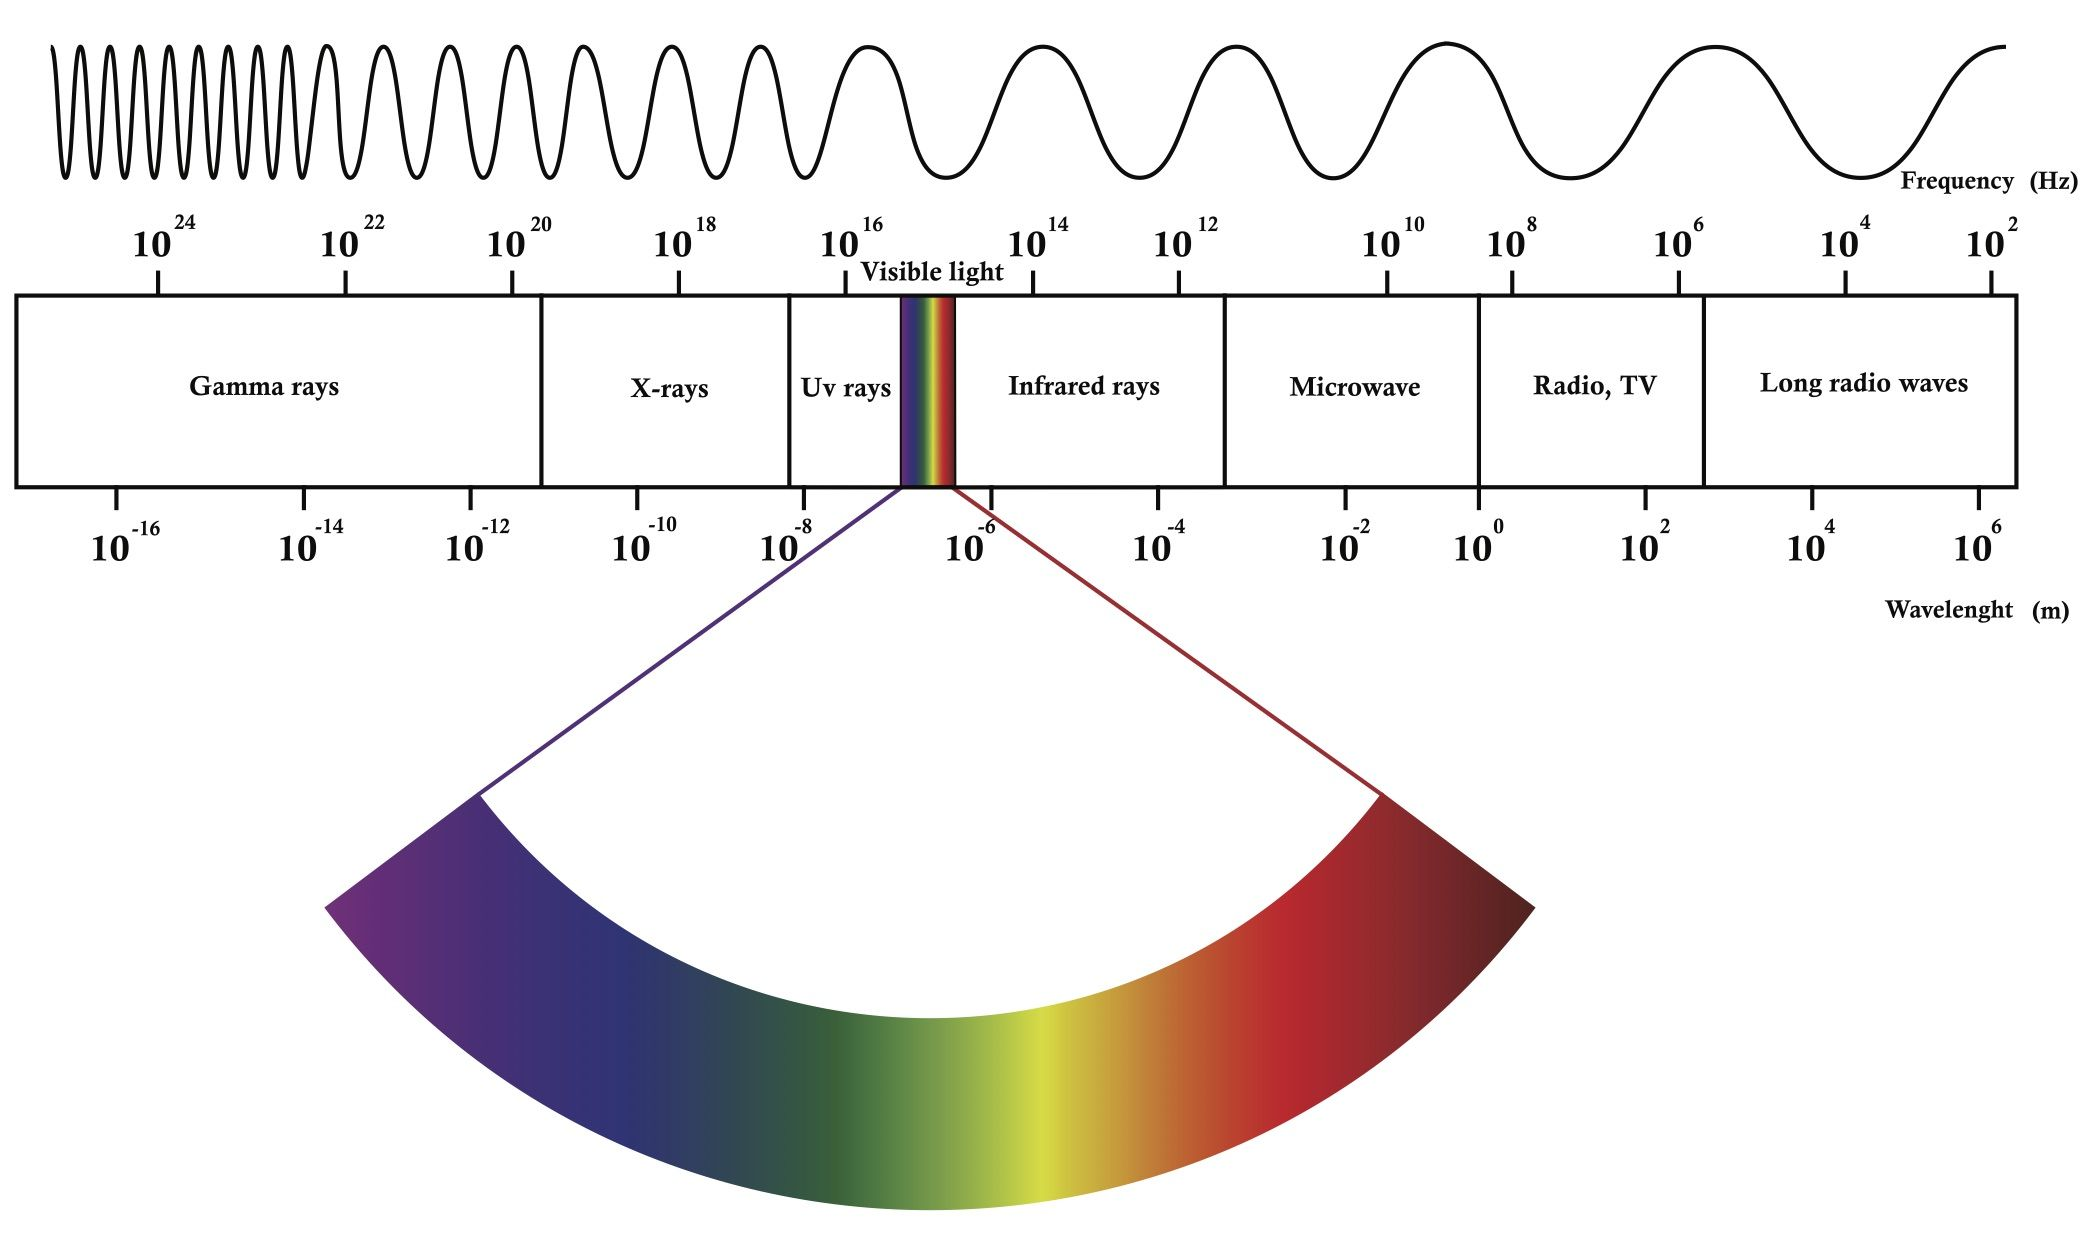
\includegraphics[width=0.7\textwidth]{images/02/spectrum.png}
    \end{tabular}
  \end{center}
  \caption{\label{fig:spectrum} Espectro eletromagnético}
  \source{\tt{https://www.livescience.com/38169-electromagnetism.html}.}
\end{figure}


%%%%%%%%%%%%%%%%%%%%%%%%%%%%%%%%%%%%%%%%%%%%%%%%%%%%%%%%%%%%
\section{Aquisição de imagens}

\begin{easylist}
& Normalmente é feita através de componentes sensíveis a alguma faixa específica do espectro eletromagnético
&& Sensores simples: fotodiodo, fototransistor.
&& Sensores lineares: CCD linear.
&& Sensores em matriz: CCD de câmeras fotográficas, mouse ótico.
\end{easylist}

\begin{figure}[!h]
  \begin{center}
    \begin{tabular}{c}
      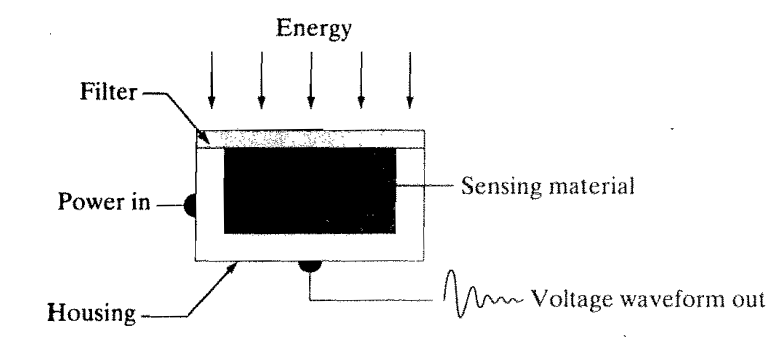
\includegraphics[width=0.8\textwidth]{images/02/sensor.png}
    \end{tabular}
  \end{center}
  \caption{\label{fig:sensor} Esquema de um sensor}
  \source{Gonzalez~\cite{gonzalez2006image}.}
\end{figure}


%%%%%%%%%%%%%%%%%%%%%%%%%%%%%%%%%%%%%%%%%%%%%%%%%%%%%%%%%%%%
\section{Amostragem e quantização}

\begin{easylist}
& Amostragem: digitalização dos valores das coordenadas, tanto no espaço quanto no tempo.
& Quantização: digitalização dos valores das amplitudes
& Representação: 
&& Matriz
\end{easylist}

  \begin{equation*}
    f(i, j) =
    \begin{bmatrix}
      f(0, 0)   & f(0, 1)   & \dots  & f(0, N-1)   \\
      f(1, 0)   & f(1, 1)   & \dots  & f(1, N-1)   \\
      \vdots    & \vdots    & \ddots & \vdots      \\
      f(M-1, 0) & f(M-1, 1) & \dots  & f(M-1, N-1) 
    \end{bmatrix}      
  \end{equation*}
    
\begin{easylist}
&& Função
\end{easylist}
  
  \begin{align*}
    & f: \mathbb{Z}^2 \rightarrow \mathbb{Z} \\
    & f: \{0, \dots, M-1\} \times \{0, \dots, N-1\} \rightarrow \{0, \dots, L-1\}
  \end{align*}

\noindent
onde $L = 2^k$. $L$ é o intervalo dinâmico do sensor e $k$ é o número de bits necessários para representar $L$.

\vspace{1cm}
  
\begin{easylist}
&& Número de bits necessários para armazenar uma imagem $M \times N$:  
\end{easylist}

\[
  b = MNk  
\]

\begin{easylist}
&& Número de bytes necessários para armazenar uma imagem $M \times N$:  
\end{easylist}

\[
  B = MNk/8  
\]



\begin{easylist}
& Redimensionamento de imagem: \textit{zoom} ou \textit{resize}
&& \textit{Nearest neighbor}: ampliar uma imagem replicando cada pixel várias vezes.
&& Bilinear: ampliar uma imagem inserindo pixels calculados da interpolação linear entre os pixels mais próximos.
\end{easylist}

%%%%%%%%%%%%%%%%%%%%%%%%%%%%%%%%%%%%%%%%%%%%%%%%%%%%%%%%%%%%
\section{Relações entre pixels}

\begin{easylist}
& Adjacência: é uma relação entre dois poxels com as propriedades listadas abaixo.
\end{easylist}

  \begin{align*}
    & 1.\; A(p, q) \Leftrightarrow x \neq y  && \text{irreflexiva} \\
    & 2.\; A(p, q) \Leftrightarrow A(q, p)   && \text{simétrica} \\
  \end{align*}
 
\begin{easylist}
&& 4-adjacência: os vizinhos de $(x, y)$ são $(x, y-1)$, $(x, y+1)$, $(x-1, y)$ e $(x+1, y)$.
&& D-adjacência: os vizinhos de $(x, y)$ são $(x-1, y-1)$, $(x-1, y+1)$, $(x+1, y+1)$ e $(x+1, y-1)$.
&& 8-adjacência: os vizinhos de $(x, y)$ são a união da 4-adjacência e da D-adjacência.
\end{easylist}

\vspace{1cm}

\begin{table}[!h]
  \centering
  \begin{tabular}{|c|c|c|}
        \hline
        $(x-1, y-1)$ & $(x, y-1)$ & $(x+1, y-1)$ \\
        \hline
        $(x-1, y  )$ & $(x, y  )$ & $(x+1, y  )$ \\
        \hline
        $(x-1, y+1)$ & $(x, y+1)$ & $(x+1, y+1)$ \\
        \hline
  \end{tabular}
  \caption{Disposição dos pixels na vizinhança de $(x, y)$.}
\end{table}


\begin{easylist}
& Distância: sejam $p$ e $q$ dois pixels pertencentes a $P$, uma distância é uma função $D:P\times P \rightarrow \mathbb{R}$ com as propriedades listadas abaixo.  
\end{easylist}

  \begin{align*}
    & 1.\; D(p, q) \geq 0 \\
    & 2.\; D(p, q) = 0 \Leftrightarrow p = q \\
    & 3.\; D(p, q) = D(q, p)                 && \text{simetria} \\
    & 4.\; D(p, q) \leq D(p, z) + D(z, q)    && \text{desigualdade triangular}    \\
  \end{align*}

\begin{easylist}
&& Distância Euclidiana:           $D_e(p, q) = \sqrt{(p_x - q_x)^2 + (p_y - q_y)^2}$
&& Distância \textit{city-block}:  $D_4(p, q) = |p_x - q_x| + |p_y - q_y|$
&& Distância \textit{chessboard}:  $D_8(p, q) = \max(|p_x - q_x|, |p_y - q_y|)$
\end{easylist}


%%%%%%%%%%%%%%%%%%%%%%%%%%%%%%%%%%%%%%%%%%%%%%%%%%%%%%%%%%%%
\section{Ferramentas matemáticas}

\begin{easylist}
& Operações lineares: seja $H$ uma operação cuja entrada e saída são imagens, sejam $f$ e $g$ duas imagens, e $a$ e $b$, dois escalares. A operação $H$ é dita linear se segue a relação abaixo

  \[
    H(af + bg) = aH(f) + bH(g)
  \]

& Operações não-lineares: uma operação é dita não-linear se não é linear.
\end{easylist}




%%%%%%%%%%%%%%%%%%%%%%%%%%%%%%%%%%%%%%%%%%%%%%%%%%%%%%%%%%%%
%Capítulo: Indentação
%%%%%%%%%%%%%%%%%%%%%%%%%%%%%%%%%%%%%%%%%%%%%%%%%%%%%%%%%%%%

%\input{indent.tex}


%%%%%%%%%%%%%%%%%%%%%%%%%%%%%%%%%%%%%%%%%%%%%%%%%%%%%%%%%%%%
%Capítulo: Entrada e saída
%%%%%%%%%%%%%%%%%%%%%%%%%%%%%%%%%%%%%%%%%%%%%%%%%%%%%%%%%%%%

%\input{io.tex}


%%%%%%%%%%%%%%%%%%%%%%%%%%%%%%%%%%%%%%%%%%%%%%%%%%%%%%%%%%%%
%Capítulo: Vetores
%%%%%%%%%%%%%%%%%%%%%%%%%%%%%%%%%%%%%%%%%%%%%%%%%%%%%%%%%%%%

%\input{array.tex}


%%%%%%%%%%%%%%%%%%%%%%%%%%%%%%%%%%%%%%%%%%%%%%%%%%%%%%%%%%%%
%Capítulo: Funções
%%%%%%%%%%%%%%%%%%%%%%%%%%%%%%%%%%%%%%%%%%%%%%%%%%%%%%%%%%%%

%\input{function.tex}


%%%%%%%%%%%%%%%%%%%%%%%%%%%%%%%%%%%%%%%%%%%%%%%%%%%%%%%%%%%%
%Capítulo: Exercícios
%%%%%%%%%%%%%%%%%%%%%%%%%%%%%%%%%%%%%%%%%%%%%%%%%%%%%%%%%%%%

%\input{exercise.tex}




%%%%%%%%%%%%%%%%%%%%%%%%%%%%%%%%%%%%%%%%%%%%%%%%%%%%%%%%%%%%
%Capítulo: Exemplos de programas
%%%%%%%%%%%%%%%%%%%%%%%%%%%%%%%%%%%%%%%%%%%%%%%%%%%%%%%%%%%%

%\chapter{Exemplos de programas}


%%%%%%%%%%%%%%%%%%%%%%%%%%%%%%%%%%%%%%%%%%%%%%%%%%%%%%%%%%%%
%Seção: pause.cpp

%\section{pause.cpp}

%\lstinputlisting[caption=series.cpp]{src/pause.cpp}

%%%%%%%%%%%%%%%%%%%%%%%%%%%%%%%%%%%%%%%%%%%%%%%%%%%%%%%%%%%%
%Seção: ascii.cpp

%\section{ascii.cpp}

%\lstinputlisting[caption=ascii.cpp]{src/ascii.cpp}

%%%%%%%%%%%%%%%%%%%%%%%%%%%%%%%%%%%%%%%%%%%%%%%%%%%%%%%%%%%%
%Seção: dado.cpp

%\section{dado.cpp}

%\lstinputlisting[caption=dado.cpp]{src/dado.cpp}

%%%%%%%%%%%%%%%%%%%%%%%%%%%%%%%%%%%%%%%%%%%%%%%%%%%%%%%%%%%%
%Seção: primos.cpp

%\section{primos.cpp}

%\lstinputlisting[caption=series.cpp]{src/primos.cpp}

%%%%%%%%%%%%%%%%%%%%%%%%%%%%%%%%%%%%%%%%%%%%%%%%%%%%%%%%%%%%
%Seção: series.cpp

%\section{series.cpp}

%\lstinputlisting[caption=series.cpp]{src/series.cpp}




%%%%%%%%%%%%%%%%%%%%%%%%%%%%%%%%%%%%%%%%%%%%%%%%%%%%%%%%%%%%
%Seção: generate.cpp

%\section{generate.cpp}

%\lstinputlisting[caption=generate.cpp]{src/generate.cpp}

%%%%%%%%%%%%%%%%%%%%%%%%%%%%%%%%%%%%%%%%%%%%%%%%%%%%%%%%%%%%
%Seção: ordena.cpp

%\section{ordena.cpp}

%\lstinputlisting[caption=ordena.cpp]{src/ordena.cpp}


\end{document}

